\documentclass[border=10pt]{standalone}
\usepackage{tikz}\usepackage{amsmath}\usetikzlibrary{arrows.meta}
\begin{document}
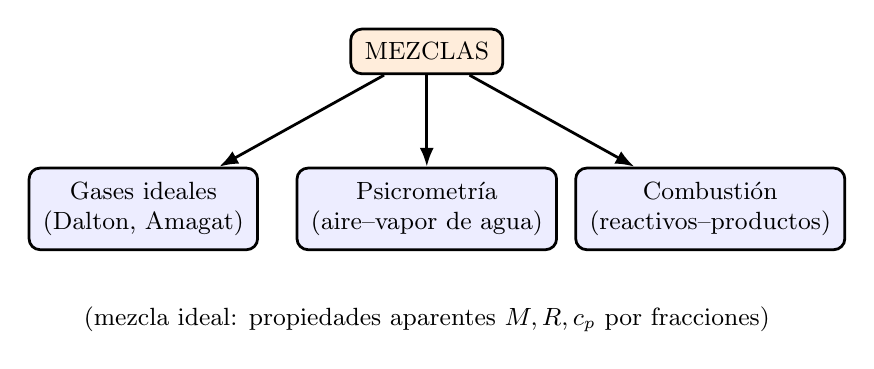
\begin{tikzpicture}[font=\small,>={Latex[length=2.4mm]},
  nd/.style={draw,line width=1pt,rounded corners,fill=blue!7,align=center,inner sep=5pt}]
  \node[nd,fill=orange!14] (m) at (0,0) {MEZCLAS};
  \node[nd] (g) at (-3.6,-2) {Gases ideales\\(Dalton, Amagat)};
  \node[nd] (p) at (0,-2) {Psicrometría\\(aire--vapor de agua)};
  \node[nd] (c) at (3.6,-2) {Combustión\\(reactivos--productos)};
  \foreach \n in {g,p,c} \draw[->,line width=1pt] (m)--(\n);
  \node[align=center] at (0,-3.4){\small (mezcla ideal: propiedades aparentes $M,R,c_p$ por fracciones)};
\end{tikzpicture}
\end{document}
